% vim: set spell spelllang=en tw=100 et sw=4 sts=4 :

\documentclass[runningheads]{llncs}

\usepackage{tikz}
\usetikzlibrary{shapes, positioning, decorations.text}

\usepackage{todonotes}

\usepackage{listings}
\lstset{
basicstyle=\small\ttfamily,
mathescape,
escapeinside={(*}{*)},
numbers=none,
keywordstyle=\bfseries\color{blue},
keywords = {language, Essence, given, letting, find, such, that,
            bool, int, matrix, enum, variant, record, set, mset,
            sequence, function, relation, partition, 
            domain, total, surjective, be,
            forAll, exists, sum, injective, in, preImage, range,
            new, type, intersect, union, from,
            minimising, maximising, of, indexed, by, and,
            defined, maxSize, maxNumParts, size, regular, language, cheese
            }
showstringspaces=false,
tabsize=1,
breaklines=true,
breakatwhitespace=false,
}

%\usepackage{showframe}

\title{Finding Subgraphs With Side Constraints\thanks{This research was supported by the
Engineering and Physical Sciences Research Council [grant number EP/P026842/1]}}

\author{
    \"Ozg\"ur Akg\"un\inst{1} \and Jessica Enright\inst{2} \and Christopher
    Jefferson\inst{1} \and Ciaran McCreesh\inst{2} \and Patrick
    Prosser\inst{3} \and Steffen Zschaler\inst{4} \\
}
\authorrunning{\"O. Akgun et al.}
\institute{
    University of St Andrews, Scotland \and
    University of Glasgow, Scotland \\ \email{ciaran.mccreesh@glasgow.ac.uk} \and
    Algorithmicists Anonymous, Scotland \and
    King's College London, England
}

\usepackage{hyperref}
\usepackage{cleveref}

\crefname{Figure}{Figure}{Figures}
\crefname{figure}{figure}{figures}

\begin{document}

\maketitle

\begin{abstract}
    The subgraph isomorphism problem is to find a small ``pattern'' graph inside a larger ``target''
    graph. There are excellent dedicated solvers for this problem, but they require substantial
    programming effort to handle complex side constraints; however, general purpose constraint
    solvers struggle on more difficult graph instances. We show how to combine the state of the art
    Glasgow Subgraph Solver with the Minion constraint programming solver to get a ``subgraphs modulo
    theories'' solver that is both performant and flexible. We also show how such an approach can be
    driven by the Essence high level modelling language, giving ease of modelling to non-expert
    users. We give practical examples involving
    temporal graphs, typed graphs from software engineering, and costed subgraph isomorphism
    problems.
\end{abstract}

\section{Introduction}

Finding or counting small ``pattern'' graphs inside larger ``target'' graphs are widely applicable
hard problems, with applications including ??. This has led to the development of numerous dedicated
algorithms, with the Glasgow Subgraph Solver \cite{DBLP:conf/gg/McCreeshP020} being the current
state of the art \cite{DBLP:conf/gbrpr/Solnon19}. However, practitioners are often interested in
versions of the problem with additional restrictions, or side constraints. Some of these, such as
exact vertex labelling schemes, are trivial to include in a dedicated solver, but others currently
require either extensive programming or inefficient post-processing. This paper explores a different
approach: by allowing the Glasgow Subgraph Solver to use the Minion constraint programming (CP) solver
\cite{DBLP:conf/ecai/GentJM06} for side constraints, we achieve both the performance only a
dedicated solver can offer, with the flexibility of a full CP toolkit. This
hybrid modelling system can be driven by the Essence high level modelling language
\cite{DBLP:journals/constraints/FrischHJHM08} and the Conjure toolchain, making it accessible to
non-specialists.

\subsection{Preliminaries}

We begin with a look at the subgraph isomorphism problem, from a high level constraint modelling
perspective.  The basic non-induced subgraph isomorphism problem is to find an injective mapping
from a pattern graph to a target graph, such that adjacent vertices in the pattern are mapped to
adjacent vertices in the target. Variations on the problem are common, and are often combined. For
example, in the induced version of the problem, non-edges must be mapped to non-edges; in the
directed version, the input graphs have directed edges whose orientations must be preserved by the
mapping; in the vertex labelled version, each vertex has a label, and the mapping must map vertices
to like-labelled vertices; and in the edge-labelled version, edges have labels which must be
preserved.  It is also common to want to count or enumerate all solutions, rather than deciding
whether at least one solution exists.  Subsets of these variations are supported by many
dedicated subgraph isomorphism algorithms, including the Glasgow Subgraph Solver.

\begin{figure}[tb]
    \centering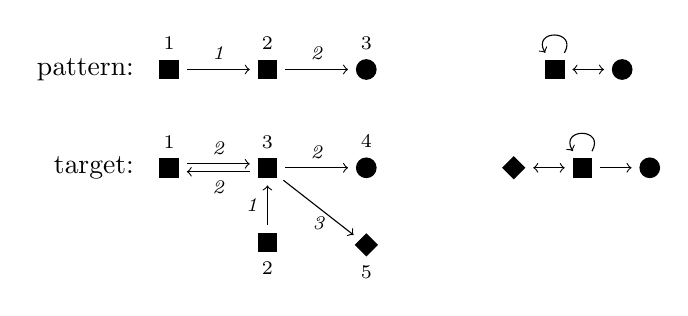
\begin{tikzpicture}
        \node [draw, fill] (P1) {}; \node [above=0cm of P1, font=\scriptsize] { 1 };
        \node [draw, fill, right=1cm of P1] (P2) {}; \node [above=0cm of P2, font=\scriptsize] { 2 };
        \node [draw, fill, circle, right=1cm of P2, inner sep=2.5pt] (P3) {}; \node [above=0cm of P3, font=\scriptsize] { 3 };
        \draw [->, shorten >=1mm, shorten <=1mm] (P1) -- (P2) node [midway, font=\scriptsize\itshape, above] { 1 };
        \draw [->, shorten >=1mm, shorten <=1mm] (P2) -- (P3) node [midway, font=\scriptsize\itshape, above] { 2 };
        \node [left=0.2cm of P1, anchor=east] { pattern: };

        \node [draw, fill, right=4.65cm of P1] (PT1) {};
        \node [draw, fill, circle, inner sep=2.5pt, right=0.6cm of PT1] (PT2) {};
        \draw [<->, shorten >=1mm, shorten <=1mm] (PT1) -- (PT2);
        \draw [->, shorten >=1mm, shorten <=1mm] (PT1) to [out=60, in=120, looseness=8] (PT1);

        \node [draw, fill, below=1cm of P1] (T1) {}; \node [above=0cm of T1, font=\scriptsize] { 1 };
        \node [draw, fill, right=1cm of T1] (T3) {}; \node [above=0cm of T3, font=\scriptsize] { 3 };
        \node [draw, fill, below=0.7cm of T3] (T2) {}; \node [below=0cm of T2, font=\scriptsize] { 2 };
        \node [draw, fill, circle, right=1cm of T3, inner sep=2.5pt] (T4) {}; \node [above=0cm of T4, font=\scriptsize] { 4 };
        \node [draw, fill, diamond, below=0.7cm of T4, inner sep=2pt] (T5) {}; \node [below=0cm of T5, font=\scriptsize] { 5 };
        \draw [->, shorten >=1mm, shorten <=1mm, transform canvas={yshift=0.5mm}] (T1) -- (T3) node [midway, font=\scriptsize\itshape, above] { 2 };
        \draw [<-, shorten >=1mm, shorten <=1mm, transform canvas={yshift=-0.5mm}] (T1) -- (T3) node [midway, font=\scriptsize\itshape, below] { 2 };
        \draw [->, shorten >=1mm, shorten <=1mm] (T2) -- (T3) node [midway, font=\scriptsize\itshape, left] { 1 };
        \draw [->, shorten >=1mm, shorten <=1mm] (T3) -- (T4) node [midway, font=\scriptsize\itshape, above] { 2 };
        \draw [->, shorten >=1mm, shorten <=1mm] (T3) -- (T5) node [midway, font=\scriptsize\itshape, below] { 3 };
        \node [left=0.2cm of T1, anchor=east] { target: };

        \node [draw, fill, right=5cm of T1] (TT1) {};
        \node [draw, fill, circle, inner sep=2.5pt, right=0.6cm of TT1] (TT2) {};
        \node [draw, fill, diamond, inner sep=2pt, left=0.6cm of TT1] (TT3) {};
        \draw [->, shorten >=1mm, shorten <=1mm] (TT1) -- (TT2);
        \draw [<->, shorten >=1mm, shorten <=1mm] (TT1) -- (TT3);
        \draw [->, shorten >=1mm, shorten <=1mm] (TT1) to [out=60, in=120, looseness=8] (TT1);
    \end{tikzpicture}
    \caption{A small pattern and a larger target graph used in examples throughout this paper. The
    plain text numbers are vertex names, and the shapes on vertices represent vertex labels. The
    graphs to the right are \emph{type graphs}, which are used in \cref{section:typegraphs}. The
    italic labels on edges are used for \emph{temporal graphs}, which are discussed in
    \cref{section:temporalgraphs}, and should otherwise be ignored.}
    \label{figure:littlegraphs}
\end{figure}

We can express these problems in the Essence high level modelling language, as follows. We assume
vertices take their labels from the set $L = \{ 1\ldots\ell \}$ for some given $\ell$, and edges
from $E = \{ 1\ldots{}e \}$ (and so $\ell$ and / or $e$ may be 1, for applications that do not use
labels on vertices and / or edges):
\begin{lstlisting}
given l, e : int
letting L be domain int(1..l)
letting E be domain int(1..e)
\end{lstlisting}
We take as input a pattern directed graph which has $p$ vertices (which we number from 1 to $p$, in
the set $P$), and a target directed graph which has $t$ vertices (numbered from 1 to $t$, the set
$T$). Each graph is represented as total function from vertices to vertex labels, and a
\emph{partial} function from pairs of (not necessarily distinct) vertices to edge labels:
\begin{lstlisting}
given p, t : int
letting P be domain int(1..p)
letting T be domain int(1..t)

given pat : function (P, P) --> E
given tgt : function (T, T) --> E
given plab : function (total) P --> L
given tlab : function (total) T --> L
\end{lstlisting}
Now we wish to find an injective mapping $f$:
\begin{lstlisting}
find f : function (total, injective) P --> T
\end{lstlisting}
that preserves vertex labels,
\begin{lstlisting}
such that forAll a : P .  plab(a) = tlab(f(a))
\end{lstlisting}
and directed edges, including their labels:
\begin{lstlisting}
such that forAll ((a, b), lbl) in pat .
    ((f(a), f(b)), lbl) in toSet(tgt)
\end{lstlisting}

As a simple example, the following inputs show the problem instance represented in
\cref{figure:littlegraphs}. We have three different vertex labels (circle, square, and diamond), and
only a single edge type (which is directed; the numerical labels on edges are not used in this
section):
\begin{lstlisting}
letting l be 3
letting e be 1
\end{lstlisting}
We may now describe the pattern:
\begin{lstlisting}
letting p be 3
letting pat be function ((1, 2) --> 1, (2, 3) --> 1)
letting plab be function (1 --> 1, 2 --> 1, 3 --> 2)
\end{lstlisting}
and the target:
\begin{lstlisting}
letting t be 5
letting tgt be function ((1, 3) --> 1, (3, 1) --> 1,
  (2, 3) --> 1, (3, 4) --> 1, (3, 5) --> 1)
letting tlab be function (1 --> 1, 2 --> 1, 3 --> 1,
  4 --> 2, 5 --> 3)
\end{lstlisting}
Using the Conjure tool to compile Essence to a constraint programming model which is then solved by
Minion, we find there are exactly two solutions to the problem, as we would expect:
\begin{lstlisting}
(1 --> 1, 2 --> 3, 3 --> 4)
(1 --> 2, 2 --> 3, 3 --> 4)
\end{lstlisting}
But what if our application requires induced isomorphisms? Then we can easily add the constraint
\begin{lstlisting}
such that forAll (a, b) : (P, P) .
    (f(a), f(b)) in defined(tgt) -> (a, b) in defined(pat)
\end{lstlisting}
And Conjure will now find us a single solution,
\begin{lstlisting}
(1 --> 2, 2 --> 3, 3 --> 4)
\end{lstlisting}
As we will see in \cref{section:problems}, supporting other problem variants and constraints is
similarly straightforward, even if auxiliary variables are required. %For example, if instead we
%want to allow relabelling on vertex labels (which
%is typically not supported by dedicated solvers), we could do the following:
%\begin{lstlisting}
%find r : function (total, injective) L --> L
%such that forAll a : P .  r(plab(a)) = tlab(f(a))
%\end{lstlisting}
%and we would find two additional solutions,
%\begin{lstlisting}
%(1 --> 1, 2 --> 3, 3 --> 5)
%(1 --> 2, 2 --> 3, 3 --> 5)
%\end{lstlisting}
%and if we removed the injective keyword for the relabelling, we would find a fifth mapping
%\begin{lstlisting}
%(1 --> 2, 2 --> 3, 3 --> 1)
%\end{lstlisting}
%We return to relabelling in \cref{section:typegraphs}.

\subsection{Preliminary Experiments and Motivation}

\begin{figure}[tb]
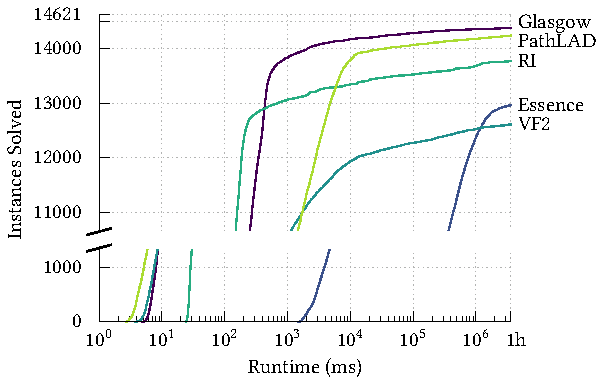
\includegraphics{gen-graph-glasgow-versus-minion-cumulative.pdf}\hfill\includegraphics*{gen-graph-glasgow-versus-minion-scatter.pdf}

    \caption{Left, the cumulative number of instances solved over time, for the non-induced decision
    problem with no side constraints. Right, comparing the high level approach with the Glasgow
    Subgraph Solver on an instance by instance basis; points on the outer axes represent
    timeouts.}\label{figure:solvers}
\end{figure}

Unfortunately, whilst elegant and flexible, the performance of this approach is rather terrible on
basic subgraph isomorphism instances.  The computational experiments in this paper are performed on
a cluster of machines with dual Intel Xeon E5-2697A v4 processors and 512GBytes RAM running Ubuntu
18.04.  Initially, we will be using the 14,621 unlabelled, undirected instances from Solnon's
benchmark suite\footnote{https://perso.liris.cnrs.fr/christine.solnon/SIP.html}. This benchmark
suite was originally designed for algorithm portfolios work \cite{DBLP:conf/lion/KotthoffMS16}, and
brings together several collections of application and randomly-generated instances with varying
difficulties and solution counts (including many unsatisfiable instances). Some of the instances
have up to 900 vertices and 14,420 edges in patterns and up to 6,671 vertices and 209,000 edges in
targets. These lead to rather large models, by constraint programming standards: the largest
generated table constraint has nearly half a million entries.

In \cref{figure:solvers} we plot the cumulative number of instances solved over time for the
non-induced decision problem, comparing the high level approach to the Glasgow Subgraph Solver
\cite{DBLP:conf/gg/McCreeshP020} and PathLAD \cite{DBLP:conf/lion/KotthoffMS16} (the two strongest
CP approaches), and to VF2 \cite{DBLP:journals/pami/CordellaFSV04} and RI
\cite{DBLP:journals/bmcbi/BonniciGPSF13} (simpler algorithms which perform well on easy instances).
The high level approach has very slow startup times (which is to be expected as it involves
launching a Java virtual machine and reading in a very large table constraint), but much more
worryingly, only catches up with the worst other solver in number of instances solved as the timeout
approaches. Worse, as the scatter plot in \cref{figure:solvers} shows, there are almost no instances
where the high level approach does better than the Glasgow Subgraph Solver. (For induced problems,
the results are even less favourable.)

These first results motivate the remainder of this paper. We want to retain the convenience of the
high level modelling approach, and to be able to add arbitrary side constraints to suit different
applications, but we do not want to have to abandon the performance that dedicated solvers can get
on hard instances. In \cref{section:hybrid} we evaluate several ways of using a CP solver in
conjunction with the Glasgow Subgraph Solver, with a focus on low level implementation details. In
\cref{section:problems} we then return to high level modelling, and look at the convenience it
provides for ??temporal problems, ??relabelling and retyping, and ??optimisation problems.

\section{Hybrid Solving}\label{section:hybrid}

The Glasgow Subgraph Solver \cite{DBLP:conf/gg/McCreeshP020} employs a CP approach to solve
subgraph-finding problems, but using special data structures and algorithms---for example, rather
than representing the adjacency constraint using a table, it uses bitset adjacency matrices
\cite{DBLP:conf/cp/McCreeshP15}. The solver also exploits various graph invariants involving degrees
\cite{DBLP:journals/constraints/ZampelliDS10} and paths \cite{DBLP:conf/cp/AudemardLMGP14} to
further reduce the search space, and employs special search order heuristics
\cite{DBLP:conf/cpaior/ArchibaldDHMP019}. From this paper's perspective, the most important design
aspect is that internally, the solver has a CP style variable for each vertex in the pattern graph,
whose domains range over the vertices of the target graph. The solver performs a backtracking search
with restarts and nogood recording, attempting to assign each variable a value from its domain,
whilst respecting adjacency and injectivity constraints. At each recursive call of search, the
solver performs \emph{propagation} to eliminate infeasible values from domains. If any domain
becomes empty, the solver backtracks; otherwise, it selects a variable, and tries assigning it each
value from its domain in turn.

For now we will assume that there is some way of setting up the subgraph solver and a CP solver such
that they both have this same set of variables and values, and that there is some way of knowing how
to form a correspondence between their internal representations. We will allow the CP solver to have
additional variables that the subgraph solver does not know about, and we do not specifically
require the CP solver to be aware of all of the graph constraints. We could therefore use a CP
solver as a \emph{solution checker}. Whenever the subgraph solver finds a solution, it will pass it
to the CP solver, which will treat the solution as a set of equality constraints. The CP solver will
then attempt to find a satisfying assignment. If the CP solver does not have any additional
variables, this is equivalent to simply checking that the remaining constraints hold, but otherwise
it can involve search. For a decision problem, the CP solver then communicates back to the subgraph
solver either ``yes, this is a valid solution'', or ``no, reject this solution and keep going''. If
we are solving a counting or enumeration problem, the CP solver must find \emph{all} solutions and
communicate this back to the subgraph solver.

For more power, but possibly also greater cost, we could additionally ask a CP solver at every stage
of search to test whether the state the subgraph solver is in is obviously infeasible.  Whenever the
subgraph solver has finished performing propagation, it can communicate the \emph{trail} (that is,
its current sequence of guessed assignments) to the CP solver, which again treats these as
additional equality constraints. The CP solver then performs its own propagation (but not search),
and communicates back either a ``yes, keep going'' or a ``no, backtrack immediately''.  Finally,
after this testing, we could also ask the CP solver to communicate any deletions it infers back to
the subgraph solver. In other words, the subgraph solver would use the CP solver as an additional
propagator.

Unfortunately, each of these approaches has drawbacks. The solution we will settle upon is based
upon \emph{rollbacks}; we will describe this below, after presenting experiments that demonstrate
the difference between these approaches.

\subsection{Implementation}

To enable communication between the two solvers, we use FIFOs (named pipes), and a simple text-based
protocol.  Both solvers are run and initialised, and then the subgraph solver proceeds as normal,
whilst the CP solver waits to be given commands. The subgraph solver thens communicate its trail
or a candidate solution as a set of assignment constraints, which the CP solver reads. The CP solver
clones its initial model, adds in the given set of constraints, and then either propagates or
searches as directed. It then communicates its success or failure state, and any deletions, back to
the subgraph solver. This approach is reasonably solver-agnostic, and adding support for different
CP solvers (or non-CP solvers) should not be difficult.

Problems specified in Essence are converted to concrete models that can be solved by a CP solver like Minion using Conjure and Savile Row.
Running Conjure with a special flag (--graph-solver) instructs it to generate an extra file for the consumption of the graph solver, in addition to a CP model written in Essence Prime.
The model is then converted to Minion input. The graph solver file includes the mappings between the nodes and the edges in the graph to the names of the decision variables used in the model. 

\subsection{Design Experiments}

\begin{figure}[p]
    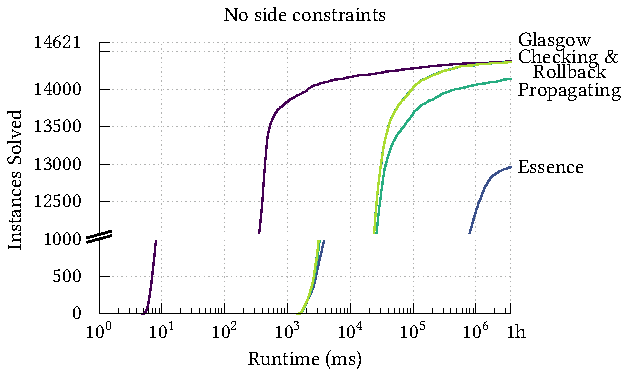
\includegraphics{gen-graph-nosideconstraints.pdf}\hfill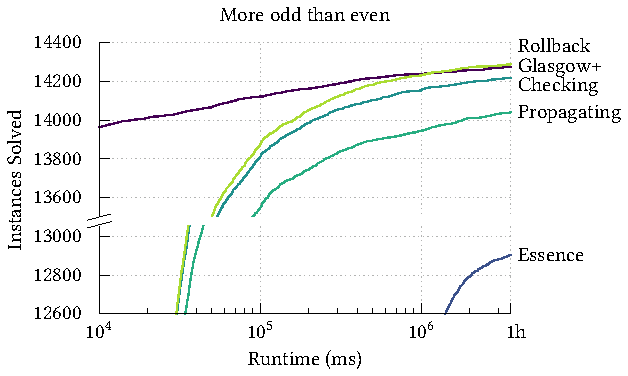
\includegraphics{gen-graph-oddeven.pdf}
    \bigskip
    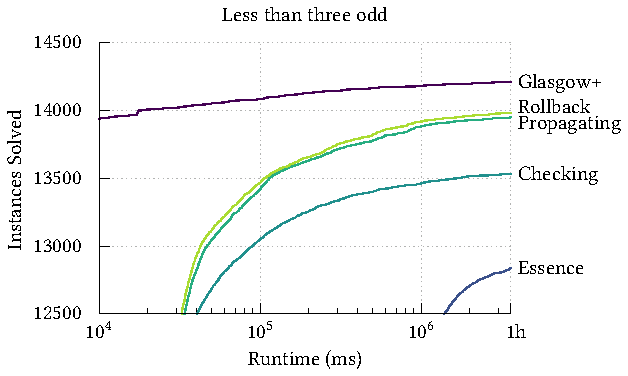
\includegraphics{gen-graph-mostlyodd.pdf}\hfill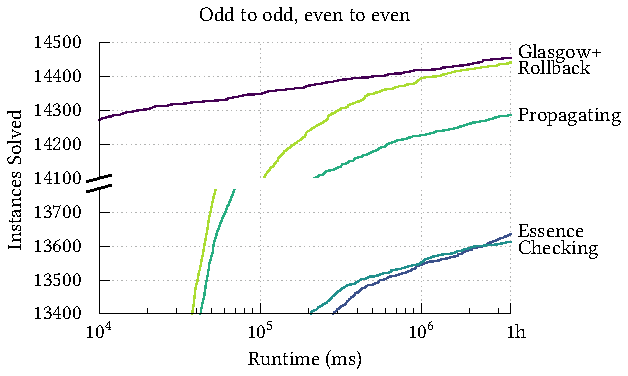
\includegraphics{gen-graph-parity.pdf}
    \caption{Comparing different approaches to hybrid solving, showing the cumulative number of
    instances solved over time. On the top row, ``no side constraints'' then with the ``more odd
    target vertices than even target vertices'' side constraint; on the bottom row, the ``mostly odd
    target vertices'' side constraint on the left, and the ``odd to odd, even to even'' side
    constraint on the right. In the top left plot, the ``Checking'' and ``Rollback'' lines are
    indistinguishable.}\label{figure:cumulative}
\end{figure}

We now present the results of some computational experiments. The experiments in this section are
designed to be computationally hard, and to emphasise the difference between the approaches, rather
than to be realistic. We will continue to work with Solnon's non-induced subgraph isomorphism
benchmark instances, but will consider three variations. Firstly, we will consider the problem with
no side constraints. This is, in some sense, the worst case scenario, where we must pay the full
price of hybrid solving, but cannot get any benefit from it. Secondly, let us say that the number of
odd-indexed target vertices used must be greater than the number of even target vertices used:
\newcommand{\modsymbol}{\%}
\begin{lstlisting}
such that (sum i : P . f(i) (*\modsymbol{}*) 2) >
    (sum i : P . (f(i) + 1) (*\modsymbol{}*) 2)
\end{lstlisting}
Thirdly, let us instead say that fewer than three odd target vertices may be used:
\begin{lstlisting}
such that (sum i : P . f(i) (*\modsymbol{}*) 2) < 3
\end{lstlisting}
And fourthly, let us say that even pattern vertices must be mapped to even target vertices, and odd
pattern vertices to odd target vertices:
\begin{lstlisting}
such that forAll a : P . (a (*\modsymbol{}*) 2) = (f(a) (*\modsymbol{}*) 2)
\end{lstlisting}

We chose these last three problems because the first is likely not to be able to
perform inference until deep in a search tree (when most pattern vertices are mapped to specific
target vertices), the second is likely to be able to perform inference early in the search tree
(after a few assignments have been made, but not at the root node), and the third should propagate
only at the root node.

The results of these experiments are presented in \cref{figure:cumulative}. Let us first look at the
top left plot, where we do not actually have any side constraints. When calling the CP solver as a
solution checker, we ultimately achieve the same performance as the Glasgow Subgraph
Solver\footnote{Actually, because high level modelling can use different names for variables and
values, we get slight differences due to changes to tiebreaking in search order heuristics.},
although we can pay a substantial startup overhead. This should not be surprising: with no side
constraints, the subgraph solver runs as normal, and will perform just one call to the CP solver on
satisfiable instances. The propagating approach is over an order of magnitude slower: calling the CP
solver at every search node is clearly very expensive. (We also tried calling the CP solver to test
feasibility, without communicating deletions; this made no noticable difference to performance, and
so is not pictured.) Finally, all approaches substantially outperform using a CP solver on its own
without help from the subgraph solver.

What about the remaining three plots in \cref{figure:cumulative}, where we do have side constraints?
As we hoped, we see differences between the three plots. On the top right, where we expect the side
constraints to fire late, solution checking clearly beats propagation during search. However, on the
bottom left, where we expect side constraints to fire early, the propagating approach is much better
than solution checking. Meanwhile, on the bottom right, where our constraints fire only at the root
node, checking performs extremely poorly compared to propagating. In each case, any hybrid approach using
the subgraph solver remains much better than a pure CP approach, except that in bottom right plot
checking is slightly worse than just using the CP solver on its own.

As a point of comparison, we also implemented these three sets of side constraints natively inside
the Glasgow solver. For the ``more odd than even'' case, we did this through solution checking, for
``less than three odd'' we implemented checking during search, and for ``odd to odd, even to even''
we implemented initial domain filtering. Our implementation choices here are intended to reflect what a
reasonable programmer would do if the high level approach were not available (and we intentionally
selected side constraints that would not be too difficult to implement). In two of the three cases,
the hand-crafted code does somewhat outperform the hybrid solving, but in the ``more odd than even''
case, hybrid solving actually beats the hand-crafted dedicated solver implementation when using the
rollback approach, which we now describe.

\subsection{A Rollback Approach to Communication}

From what we have seen so far, it is obviously important to call the CP solver \emph{some} of the
time during search, but too expensive to call it \emph{all} of the time. We will therefore introduce
a new approach, which we call \emph{rollback}. This approach is inspired by backjumping ??cite, as
well as by the conflict analysis methods used in SAT and SMT solvers ??cite and in lazy clause
generating CP solvers ??cite. The idea is as follows.  Firstly, we call the CP solver with full
propagation at the root node, in case we are dealing with a particularly rich labelling scheme.
Secondly, we use the CP solver for solution checking, since this is required for correctness. Now,
suppose the CP solver rejects a candidate solution: this will cause the subgraph solver to
backtrack. At this point, we call the CP solver again, with full propagation. Either the CP solver
indicates feasibility, in which case we proceed with search (potentially with a reduced set of
domains), or the CP solver indicates failure, in which case we backtrack again, and do another
attempt at full propagation, and so on until feasiblity is reached.

The idea behind this approach is to avoid calling the CP solver when it is unlikely to do anything
useful, but that once a failure has been encountered, we want to extract as much information as we
can from the CP solver. If the failure encountered was due to a ``local'' property of the solution,
such as in the ``more odd than even'' example, then we will quickly return to just using the
subgraph solver for search. However, if the failure is due to only a few early assignments, as in
the ``fewer than three odd vertices'' example, then we will jump back to nearly the root of the
search tree.

The results in \cref{figure:cumulative} demonstrate the success of this approach. When there are no
side constraints, this approach has no overheads compared to solution checking. When constraints
fire late, this approach is better than solution checking, and when constraints fire early, this
approach is better than always propagating during search. In other words, rolling back from failures
gives us all of the strengths and none of the weaknesses of the simpler approaches. We will
therefore use this method for the remainder of the paper.

\section{Subgraph Problems with Side Constraints}\label{section:problems}

We now look at three classes of real-world subgraph-finding problems that, until now, have been
solved using dedicated approaches. We show how easy it is to model these problems in Essence. ?? do
some actual simple experiments on them?

\subsection{Retyping Problems}\label{section:typegraphs}

  In graph theory~\cite{Ehrig+06}, a graph is given by a set of vertices and a set of edges and two functions giving the source and target node for an edge, respectively.
  Morphisms between graphs map vertices to vertices and edges to edges, preserving the structure of the graphs.
  Often, we are interested in typed graphs.
  Here, we assume a dedicated graph TG---the type graph---to be given.
  Then we can define typed graphs as graphs for which a morphism into TG has been defined.
  In effect, we are labelling each vertex and edge with its corresponding type.
  
  For typed graphs, morphisms between the graphs are typically defined between graphs typed over the same type graph, but there are situations where we are interested in mapping between graphs typed over different type graphs.
  We describe an example scenario in~\cite{Duran+12,Duran+17}, where we compose graph transformation systems by defining morphisms between the rules constituting the respective transformation systems.
  In this case, the source and target transformation systems will normally have different type graphs and we will first establish a morphism between the two type graphs.
  Mappings between the various graphs making up the rules then need to preserve structure and typing subject to the morphism between type graphs.
  We have developed tool support for this approach to specification composition.\footnote{\url{https://github.com/gts-morpher/gts_morpher}}
  A key objective is to minimise the amount of specification that needs to be written.
  For example, the tool allows morphisms between graph transformation systems to be only partially specified and then automatically completes the full morphism, if it can do so unambiguously.
  This requires solving a sub-isomorphism problem.

%A \emph{typed graph} is a kind of labelled graph where the labels also carry a graph structure
%??cite. In general, mappings between typed graphs must preserve the label structure, but here we
%will be looking at a problem variation involving relabelling which occurs in ??application. 
We may describe typed graph subisomorphism problems in Essence as follows. As before, we are given a
pattern graph and a target graph, both of which carry labels; we will draw the vertex labels from
different sets, to emphasise
the relabelling.
\begin{lstlisting}
given pl, tl, e : int
letting PL be domain int(1..pl)
letting TL be domain int(1..tl)
letting E be domain int(1..e)
\end{lstlisting}
We are also given labelled graphs,
\begin{lstlisting}
given p, t : int
letting P be domain int(1..p)
letting T be domain int(1..t)

given pat : function (P, P) --> E
given tgt : function (T, T) --> E
given plab : function (total) P --> PL
given tlab : function (total) T --> TL
\end{lstlisting}
but now the labels also carry a graph structure,
\begin{lstlisting}
given pattype : function (PL, PL) --> E
given tgttype : function (TL, TL) --> E
\end{lstlisting}
We are looking for an injective mapping from the pattern graph to the target graph,
\begin{lstlisting}
find f : function
    (total, injective) P --> T
\end{lstlisting}
as well as an injective mapping between the label graphs,
\begin{lstlisting}
find r : function
    (total, injective) PL --> TL
\end{lstlisting}
in such a way that graph structure and labels are preserved,
\begin{lstlisting}
such that forAll ((a, b), lbl) in pat .
    ((f(a), f(b)), lbl) in toSet(tgt)
such that forAll a : P .
    r(plab(a)) = tlab(f(a))
\end{lstlisting}
and also requiring that the structure on the labels is preserved,
\begin{lstlisting}
such that forAll (a,b) in defined(pattype) .
    pattype((a,b)) = tgttype((r(a),r(b)))
\end{lstlisting}
?? Should we say that we are now searching for a commuting square?

Consider again the example in \cref{figure:littlegraphs}, and now suppose they are equipped with the type
structures shown to the right of each graph,
\begin{lstlisting}
letting pattype be function (
  (1, 1) --> 1, (1, 2) --> 1, (2, 1) --> 1 )
letting tgttype be function (
  (1, 1) --> 1, (1, 2) --> 1,
  (1, 3) --> 1, (3, 1) --> 1 )
\end{lstlisting}
We now find two solutions:
\begin{lstlisting}
(1 --> 1, 2 --> 3, 3 --> 5)
(1 --> 2, 2 --> 3, 3 --> 5)
\end{lstlisting}
because we can map pattern vertex 3 to target vertex 5 through retyping, but mapping pattern vertex 3
to target vertex 4 would not respect the type graph structure.

\subsection{Temporal Subgraph Problems}\label{section:temporalgraphs}
In a \emph{temporal graph}, edges are labelled with timestamps that denote times when edges are active---here we use
integers as timestamps.  Including information on the timing of edges substantially increases the modelling power of these graphs, allowing them to 
more accurately reflect the structure and dynamics of a wide variety of real-world systems (e.g. trade networks, changing contact networks, transport networks), 
and address optimisation questions in which the timing of edges is fundamental.  

As algorithms and formalisms have become available for temporal graphs, examples of their application have become widespread \cite{holmeReview}, 
notably including applications within epidemiology \cite{temporalEpi} and computational social science \cite{socialTemporalCite}.
Because the use of temporal graphs has spread beyond theoretical researchers, the ability to rapidly define and experiment with 
new problem definitions and constraints is valuable - practitioners are unlikely to define bespoke algorithms for novel problems as they arise.

%Temporal graphs 
% why being able to try new constraints easily is useful for practitioners

%In a \emph{temporal graph}, edges are labelled with some kind of timestamp---here we will use
%integers. Temporal pattern matching and counting has applications in ??. 
There are at least three
common kinds of temporal subgraph isomorphism. In an \emph{exact} subisomorphism, times are simply
labels that must match exactly. If we look at \cref{figure:littlegraphs}, now ignoring vertex labels
but using the edge labels to carry the timestamps,
\begin{lstlisting}
letting l be 1
letting e be 3

letting p be 3
letting pat be function ((1, 2) --> 1, (2, 3) --> 2)
letting plab be function (1 --> 1, 2 --> 1, 3 --> 1)

letting t be 5
letting tgt be function ((1, 3) --> 2, (3, 1) --> 2,
  (2, 3) --> 1, (3, 4) --> 2, (3, 5) --> 3)
letting tlab be function (1 --> 1, 2 --> 1, 3 --> 1,
  4 --> 1, 5 --> 1 )
\end{lstlisting}
then there are two solutions,
\begin{lstlisting}
(1 --> 2, 2 --> 3, 3 --> 1)
(1 --> 2, 2 --> 3, 3 --> 4)
\end{lstlisting}

A less strict kind of subisomorphism is an \emph{offset}, where edge labels must match exactly but
offset by an integer constant. In our example, this means ``find a mapping where the event from 2
to 3 occurs one time unit after the event from 1 and 2''. We can model this as follows:
\begin{lstlisting}
find o : int(-e..e)
such that forAll (a,b) in defined(pat) .
    pat((a,b)) = o + tgt((f(a), f(b)))
\end{lstlisting}
and we find one additional solution,
\begin{lstlisting}
(1 --> 1, 2 --> 3, 3 --> 5)
\end{lstlisting}

Finally, in an \emph{order} embedding, the pattern edge labels simply define an order on events. We
can model this as follows:
\begin{lstlisting}
find o : function (total) E --> E
such that forAll x : int(1..e - 1) .  o(x) <= o(x + 1)
such that forAll (a,b) in defined(pat) .
    pat((a,b)) = o(tgt((f(a), f(b))))
\end{lstlisting}
which gets us yet another solution,
\begin{lstlisting}
(1 --> 2, 2 --> 3, 3 --> 5)
\end{lstlisting}

Of course, when using a high level modelling approach, we are not restricted to these three problem
variants, and could easily try out new models in an interactive setting. For example, it would take
only a few minutes to write a model for a temporal problem where all edges must occur within a short
but unspecified time period, whereas adapting a dedicated solver to check this constraint would be a
substantial programming effort (and making the solver propagate rather than check this constraint
would be even harder).

\subsection{Subgraph Isomorphism With Costs}

The system we created also support optimisation problems (and does not require that the subgraph
isomorphism solver be aware that this is what is going on). If, for example, each target vertex has
a cost associated with it,
\begin{lstlisting}
given tcost : function (total) T --> int
\end{lstlisting}
then we can ask to find the cheapest solution,
\begin{lstlisting}
minimising sum([ tcost(f(a)) | a : P])
\end{lstlisting}
We could also just as easily ask for the solution whose most expensive edge is cheapest, or that
uses fewest vertices with a particular label. These kinds of problem occur widely in practice,
including in ?? skyline graphs, ?? labelled subgraph finding, ?? weighted cliques.

\section{Conclusion}

?? A lot of flexibility, decent performance on hard instances although the startup costs are
vicious. A key benefit is supporting large queries, which current solutions struggle with. Suitable
for interactive use in domain settings. For integration into larger systems, would benefit from
bypassing the high level modelling language and using two low level solvers directly.

\bibliographystyle{splncs04}
\bibliography{paper}

\end{document}

